\documentclass{article}

\usepackage{corl_2026}
\usepackage{booktabs}
\usepackage{graphicx}
\usepackage{amsmath}

\title{Recalibrate After You Accelerate: Few-Step Flow Sampling Silently Disarms a VLA's Failure Monitors}

\author{Anonymous}

\begin{document}
\maketitle

\begin{abstract}
Robots controlled by vision-language-action (VLA) models are often paired with a failure
monitor: a lightweight check that raises an alarm when a task seems to be going wrong. The
monitor's alarm threshold is tuned on the model as originally trained, but the model that gets
deployed is usually a sped-up version, so we ask whether the monitor still works after that
swap. We tune four common monitors on the open SmolVLA model, then run sped-up versions of it in
the LIBERO-Long simulator with the monitors left unchanged. The most practical speed-up, building
each action plan in 2 refinement steps instead of 10, makes the model 2.5$\times$ faster and
just as successful. Yet it disables a monitor that watches the robot's planned actions: it caught
about half of all failures before and catches none after, because the faster model's successive
plans agree more closely, which pulls its scores below the old threshold. Checking false alarms,
the only thing the monitor's tuning guarantees, cannot reveal this, since false alarms drop to
zero too. Compressing the model's weights has a mirror-image effect on a monitor that reads the
model's visual and language features, pushing it toward reporting ``safe'' as compression
increases. Whenever a robot policy is sped up, its monitor should be re-tuned and tested on real
failures.
\end{abstract}

\keywords{VLA, acceleration, quantization, runtime monitoring, conformal prediction}

\section{Introduction}

A \emph{failure monitor} watches a robot while it works and raises an alarm when the current
attempt looks likely to fail, so that a person or a fallback controller can step in. For robots
driven by vision-language-action (VLA) models, a monitor is usually a small scoring function that
reads either the model's internal state or the actions it plans. The function gives every step a
score, and an alarm fires when the score crosses a threshold~\citep{safe,vlafail,fiper,sentinel}.
The threshold is set from runs of the policy as trained. A common recipe uses only successful
runs, choosing the threshold so that at most a fixed fraction of them, say 10\%, would ever raise
an alarm~\citep{safe,fiper,sentinel}. This is a conformal guarantee~\citep{conformal}. It limits
false alarms, but it holds only if the deployed policy behaves like the one the threshold was
tuned on, and it promises nothing about how many failures get caught.

The policy that is actually deployed is rarely the policy as trained. To run fast enough on a
robot, it is sped up by storing its weights with fewer bits (quantization), by pruning, or by
cutting the number of steps it takes to produce each action~\citep{vlaquantbench,quantvla,care}.
Papers on these speed-ups check that the robot still succeeds, but the monitor is typically
carried over unchanged. For language-model monitors, model updates cause recoverable drift rather
than erasing the signal, and quantization leaves the monitor's ranking accuracy largely
intact~\citep{duan}. Concurrent work finds that a VLA monitor's scores shift under 4-bit weights
while its ranking holds, replaying the original policy's recorded observations through the
compressed model~\citep{rankpreserving}.

We test the deployed setup directly. We run each sped-up policy on the robot task itself, so the
robot's own actions decide what it sees next, and four unchanged monitors watch it. With 2
action-refinement steps instead of 10, the robot succeeds as often, but one monitor stops catching
failures entirely and a second catches fewer; monitors that read the visual and language features
are unaffected. The usual check cannot see this, because the broken monitors raise \emph{fewer}
false alarms, the only thing their threshold controls. Weight compression does the opposite,
pushing a monitor that reads the visual and language features toward reporting ``safe''.

\section{Setup}
\label{sec:setup}

\paragraph{Robot policy and task.} SmolVLA~\citep{smolvla} is an open VLA with ${\sim}$450M parameters. A
  vision-language backbone (SmolVLM-2) reads the camera images and the instruction. An
  \emph{action expert} then plans the next 50 actions, building the plan from random noise in 10
  refinement steps (flow matching). The robot executes the first action and replans at the next
  step. We use the public LIBERO checkpoint with its own settings, run through LeRobot, and
evaluate on LIBERO-Long~\citep{libero}, a simulated suite of 10
  long-horizon manipulation tasks. Each episode starts from one of 50 fixed initial states per task
and is a failure if the task is not done within 520 steps. The original policy succeeds in 32\% of 500 episodes, below the
  71\% the SmolVLA paper reports. A public reproduction of this checkpoint reports
  56\%.\footnote{\url{https://github.com/huggingface/lerobot/issues/3264}} Our rollout code
matches the success rate of LeRobot's own evaluator on the same task and initial states.

\paragraph{Speed-ups.} \textbf{2 refinement steps} instead of 10, with weights untouched; time
per policy call (batch of 10, one L4 GPU) falls from 0.81\,s to 0.32\,s. \textbf{Weight
quantization} rounds every weight in all 521 linear layers to 8 or 4 bits: \textbf{int8} uses one
scale per output channel, \textbf{int4-g32} one per group of 32 weights, and
\textbf{int4-coarse} groups of 128 where the layer width allows and one scale per row otherwise.
The rounding is simulated, so it reproduces low-bit accuracy but not low-bit speed.

\paragraph{Monitors.} We fit four monitors once, on runs of the original policy, and never
change them. Each is a simplified member of a published family.
\begin{itemize}
  \item \textbf{VLM probe}: a linear classifier on the backbone's final state that predicts whether
  the episode will fail (a linear version of SAFE~\citep{safe}).
  \item \textbf{Expert probe}: the same classifier on the action expert's internal state.
  \item \textbf{Mahalanobis}: how far the backbone's state lies from those seen in successful
  training runs. It needs no failure examples (after VLA-FAIL~\citep{vlafail}).
  \item \textbf{Action consistency}: how much each new 50-action plan disagrees with the previous
  one on the steps they share (after Sentinel~\citep{sentinel}).
\end{itemize}
A monitor's score at step $t$ is the average of its per-step scores so far. The alarm fires the
first time that average exceeds the threshold after a 10-step warm-up. The threshold is set on
successful runs of the original policy so that at most 10\% of them would raise an alarm.

\paragraph{Protocol.} Initial states 0--29 of every task train the monitors, 30--39 set the
thresholds, and 40--49 form the test set: 100 episodes per policy variant, all starting from the
same initial states with the same random seed. We pre-registered the hypotheses, data splits and
monitors before collecting data, and label everything else exploratory.

\section{Results}

\begin{figure}[t]
  \centering
  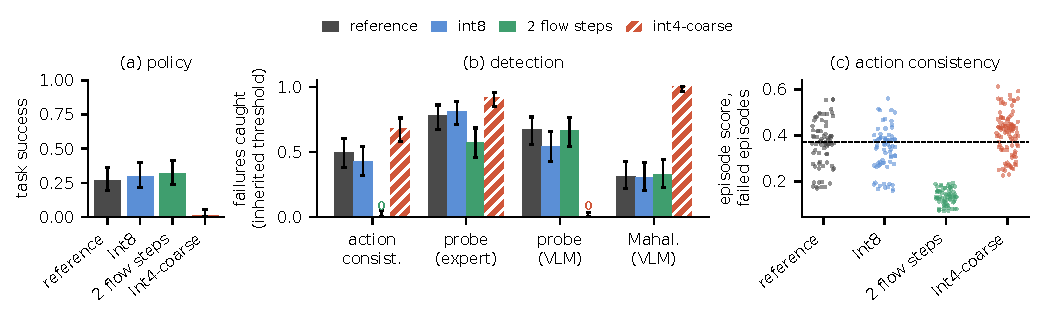
\includegraphics[width=\linewidth]{fig_main.pdf}
  \vspace{-1.6em}
  \caption{\textbf{(a)} Task success of each policy variant. \textbf{(b)} The fraction of failed
  episodes each monitor catches, using the threshold set on the original policy. \textbf{(c)} The
  action-consistency monitor's scores on failed episodes. The dashed line is its threshold; with 2
  refinement steps every failure falls below it. Error bars are 95\% intervals over 100 test
  episodes per variant. Hatched bars are int4-coarse, which breaks the policy.}
  \label{fig:main}
  \vspace{-0.6em}
\end{figure}

\paragraph{The fastest setting silently disables the action monitors.} With 2 refinement steps
the robot succeeds in 32\% of test episodes, against 27\% for the original. Yet:
\begin{itemize}
  \item \textbf{Action consistency} caught 49\% of the original policy's failures (36 of 73). It
  catches none of the fast policy's 68 failures (Fig.~\ref{fig:main}b,c). Among starting positions
  where both versions fail, it misses 30 failures it used to catch and catches none it used to miss
  ($p{=}2{\times}10^{-9}$, paired McNemar test).
  \item \textbf{The expert probe} drops from 78\% to 57\% (14 lost, 0 gained, $p{=}10^{-4}$). Its
  typical alarm comes at step 124 instead of step 10.
  \item \textbf{The two monitors that read the backbone} do not change: the VLM probe catches 66\%
  against 67\%, and Mahalanobis 32\% against 32\%. Fewer refinement steps change only the action
  expert. On the first step of each episode, where both versions see the same image, the
  backbone's state is bit-for-bit identical.\footnote{On 6 of the 10 tasks, and on 19 of 20
  episodes of a seventh. On the remaining 3 tasks, GPU kernel autotuning slightly changed the
  original policy's first-step state. Excluding those tasks leaves every headline number intact.}
\end{itemize}

\begin{table}[t]
  \centering
  \small
  \setlength{\tabcolsep}{3.5pt}
  \caption{What changes when the policy goes from 10 to 2 refinement steps (original
  $\rightarrow$ fast), on the test set.
  \emph{Caught} and \emph{false alarms} use the original threshold.
  \emph{Best possible} is the most failures any threshold could catch at $\le$10\% false alarms,
  chosen with hindsight on the test set.
  \emph{AUROC} is the probability that a random failure scores above a random success.
  \emph{Re-tuned} sets a new threshold on the fast policy's own successful runs.}
  \label{tab:calib}
  \begin{tabular}{lccccc}
    \toprule
    & failures & false & best & & re-tuned: \\
    monitor & caught & alarms & possible & AUROC & caught / false al. \\
    \midrule
    action consistency & .49$\rightarrow$\textbf{.00} & .15$\rightarrow$.00 & .44$\rightarrow$.34 & .77$\rightarrow$.72 & .26 / .03 \\
    expert probe & .78$\rightarrow$\textbf{.57} & .11$\rightarrow$.00 & .77$\rightarrow$.71 & .95$\rightarrow$.94 & .66 / .06 \\
    VLM probe & .67$\rightarrow$.66 & .04$\rightarrow$.00 & .81$\rightarrow$.87 & .95$\rightarrow$.96 & .60 / .00 \\
    Mahalanobis & .32$\rightarrow$.32 & .07$\rightarrow$.06 & .36$\rightarrow$.38 & .85$\rightarrow$.86 & .29 / .06 \\
    \bottomrule
  \end{tabular}
  \vspace{-0.8em}
\end{table}

\paragraph{The scores still carry the signal; the threshold is what breaks.}
\begin{itemize}
  \item \textbf{The score shrinks by a constant factor.} With 2 steps, consecutive plans agree more
  closely. On the same starting position, action disagreement over the first 30 steps is 0.42
  times its original value (middle half of episodes: 0.40--0.44).
  \item \textbf{The ranking survives} (Table~\ref{tab:calib}). Failures still mostly score above
  successes: AUROC goes from 0.77 to 0.72. With hindsight, a threshold could still catch 34\% of
  failures.
  \item \textbf{The old threshold now sits above every score.} Re-tuning it on the fast
  policy's successful runs brings detection back to 26\%.
  \item \textbf{The failure looks like an improvement.} False alarms fall to zero, from 15\% for
  action consistency and from 11\% for the expert probe. A team that checks the false-alarm rate,
  the one thing the threshold guarantees, would see the monitor getting better.
\end{itemize}
The concurrent work reports this same pattern, rankings intact but thresholds wrong, for quantized
probes~\citep{rankpreserving}. Our result shows it also hits a monitor with no learned parameters
at all.

\paragraph{Weight quantization pushes the VLM probe toward ``safe''.}
\begin{itemize}
  \item \textbf{Score shift.} On the first step of each episode, where every variant sees the same
  image, the VLM probe's score moves toward ``safe'' by 0.29 standard deviations under int8 (in
  every episode), 2.3 under int4-g32 and 4.6 under int4-coarse.
  \item \textbf{Detection follows.} The share of failures it catches falls from 67\% to 54\% (int8:
  13 lost, 3 gained, $p{=}0.02$; exploratory), then to 9\% and to 0\%.
  \item \textbf{int8 still looks fine by the usual checks.} Task success and false-alarm rates stay
  unchanged.
  \item \textbf{The int4 settings break the policy itself} (5\% and 1\% success). Under
  int4-coarse, the probe stays silent through all 99 failures. The Mahalanobis monitor alarms on
  every int4 episode, successes included, so it is detecting the compression rather than the
  failures.
\end{itemize}

\paragraph{Checks.} \emph{Episode length:} failed episodes run to the time limit, which gives
a monitor more chances to alarm~\citep{rankpreserving}. Counting only alarms before step 200
lowers the original detection rates (VLM probe 0.67$\rightarrow$0.48, action consistency
0.49$\rightarrow$0.27), but both zeros stay at zero. \emph{Task identity:} two tasks never
succeed, so a probe could score well just by recognizing them. Within single tasks the original
AUROC is still 0.96 (VLM probe) and 0.98 (expert probe), and dropping those tasks changes no
conclusion. \emph{Pre-registration:} we predicted more false alarms under int4, which could not be
tested because int4-coarse left one successful test episode. Two secondary predictions held: 2
steps moves the expert probe more than int8 does, and int8 changes no false-alarm rate by more
than 0.05 (its AUROC prediction held for three of four monitors). We measured detection rates as planned but did not predict their collapse.

\section{Related work and discussion}

\paragraph{Related work.} VLA monitors are evaluated with the policy they were fit to held
fixed~\citep{safe,vlafail,fiper,sentinel,rescue}; SAFECAST~\citep{safecast} studies thresholds
under changes to the robot's inputs. Monitors under model updates have been studied for language
models~\citep{duan} and, concurrently, for a quantized VLA replayed on recorded
inputs~\citep{rankpreserving}. Speed-up studies measure success, speed and motion
quality~\citep{vlaquantbench,quantvla,embodiedeff,care}, not the monitor that ships with the
policy.

\paragraph{Takeaways.} Treat every speed-up as invalidating a monitor's threshold, even when
task success holds. Test the re-tuned monitor on failures of the sped-up policy, not just its
false-alarm rate. Expect a monitor to break where its input changes: the backbone monitors
survived fewer refinement steps, and the action monitors did not.

\paragraph{Limitations.} One policy, one task suite and one seed, with 100 test episodes per
variant. The original policy's success rate is low, and quantization is simulated. Our monitors
are simplified versions of the published ones; SAFE, for example, uses a threshold that varies
over time. int4-coarse was not the setting we intended; code review caught it, and we report it
under an accurate description.

\bibliography{refs}

\end{document}
